% !TeX program = lualatex
% !TeX encoding = utf8

%\documentclass{beamer}
\documentclass[aspectratio=169, smaller]{beamer}

\usepackage{amsmath}
\usepackage[T1]{fontenc}

% This is the "normal" package based install
\usepackage{lhcb_presentation/package}

\usepackage{units}
\usepackage{booktabs}
\usepackage{ulem}
\usepackage{comment}
\usepackage{listings}
\usepackage{pgfplots}

\definecolor{ACATtan}{RGB}{201,159,109}
\definecolor{ACATdtan}{RGB}{179,72,18}
\definecolor{ACATlblue}{RGB}{24,146,200}
\definecolor{ACATdgreen}{RGB}{0,68,0}
\definecolor{ACATdbrown}{RGB}{65,14,23}
\definecolor{ACATbackground}{RGB}{255, 204, 102}

\tikzstyle{ACATdark}=[fill=ACATtan, draw=ACATdbrown, ultra thick]
\tikzstyle{ACATselected}=[fill=ACATdtan, draw=ACATdbrown, ultra thick]
\tikzstyle{ACATdarktext}=[text=ACATdbrown]
\tikzstyle{ACATselectedtext}=[text=white]

% This should be appendtographicspath if using package method
\appendtographicspath{{./images/}}

\lstset{
    columns=fullflexible,
    basicstyle=\ttfamily\small,
    stringstyle=\color{green!50!black},
    keywordstyle=\color{orange},
    commentstyle=\color{white!50!black},
    emph={GooFit,Observable,DataSet,Variable,FitManager,
          goofit,GaussianPdf,DalitzPlotter},
    emphstyle=\color{blue!50!black}
}

\errorcontextlines 10000

\title{A Python upgrade to the GooFit package for parallel fitting}

\author[Henry Schreiner]{%
        Henry Schreiner\textcolor{lhcbRed}{\inst{1 }} \and
        Himadri Pandey\textcolor{lhcbRed}{\inst{1 }} \and
        Michael Sokoloff\textcolor{lhcbRed}{\inst{1 }} \and \\
        Hittle Bradley\textcolor{lhcbRed}{\inst{2 }} \and
        Karen Tomko\textcolor{lhcbRed}{\inst{2 }} \and
        Christoph Hasse\textcolor{lhcbRed}{\inst{3 }}
}
\institute{\inst{1} University of Cincinnati \and
           \inst{2} Ohio Supercomputer Center \and
           \inst{3} CERN / Technische Universitaet Dortmund (DE)}
\date{\today}

% Auto-fullscreen
% \lhcbhypersetup

\begin{document}

\begin{frame}
\titlepage
\end{frame}

\section{GooFit Introduction}
\subsection{GooFit Introduction}
\begin{frame}{Intro}
    \begin{center}
    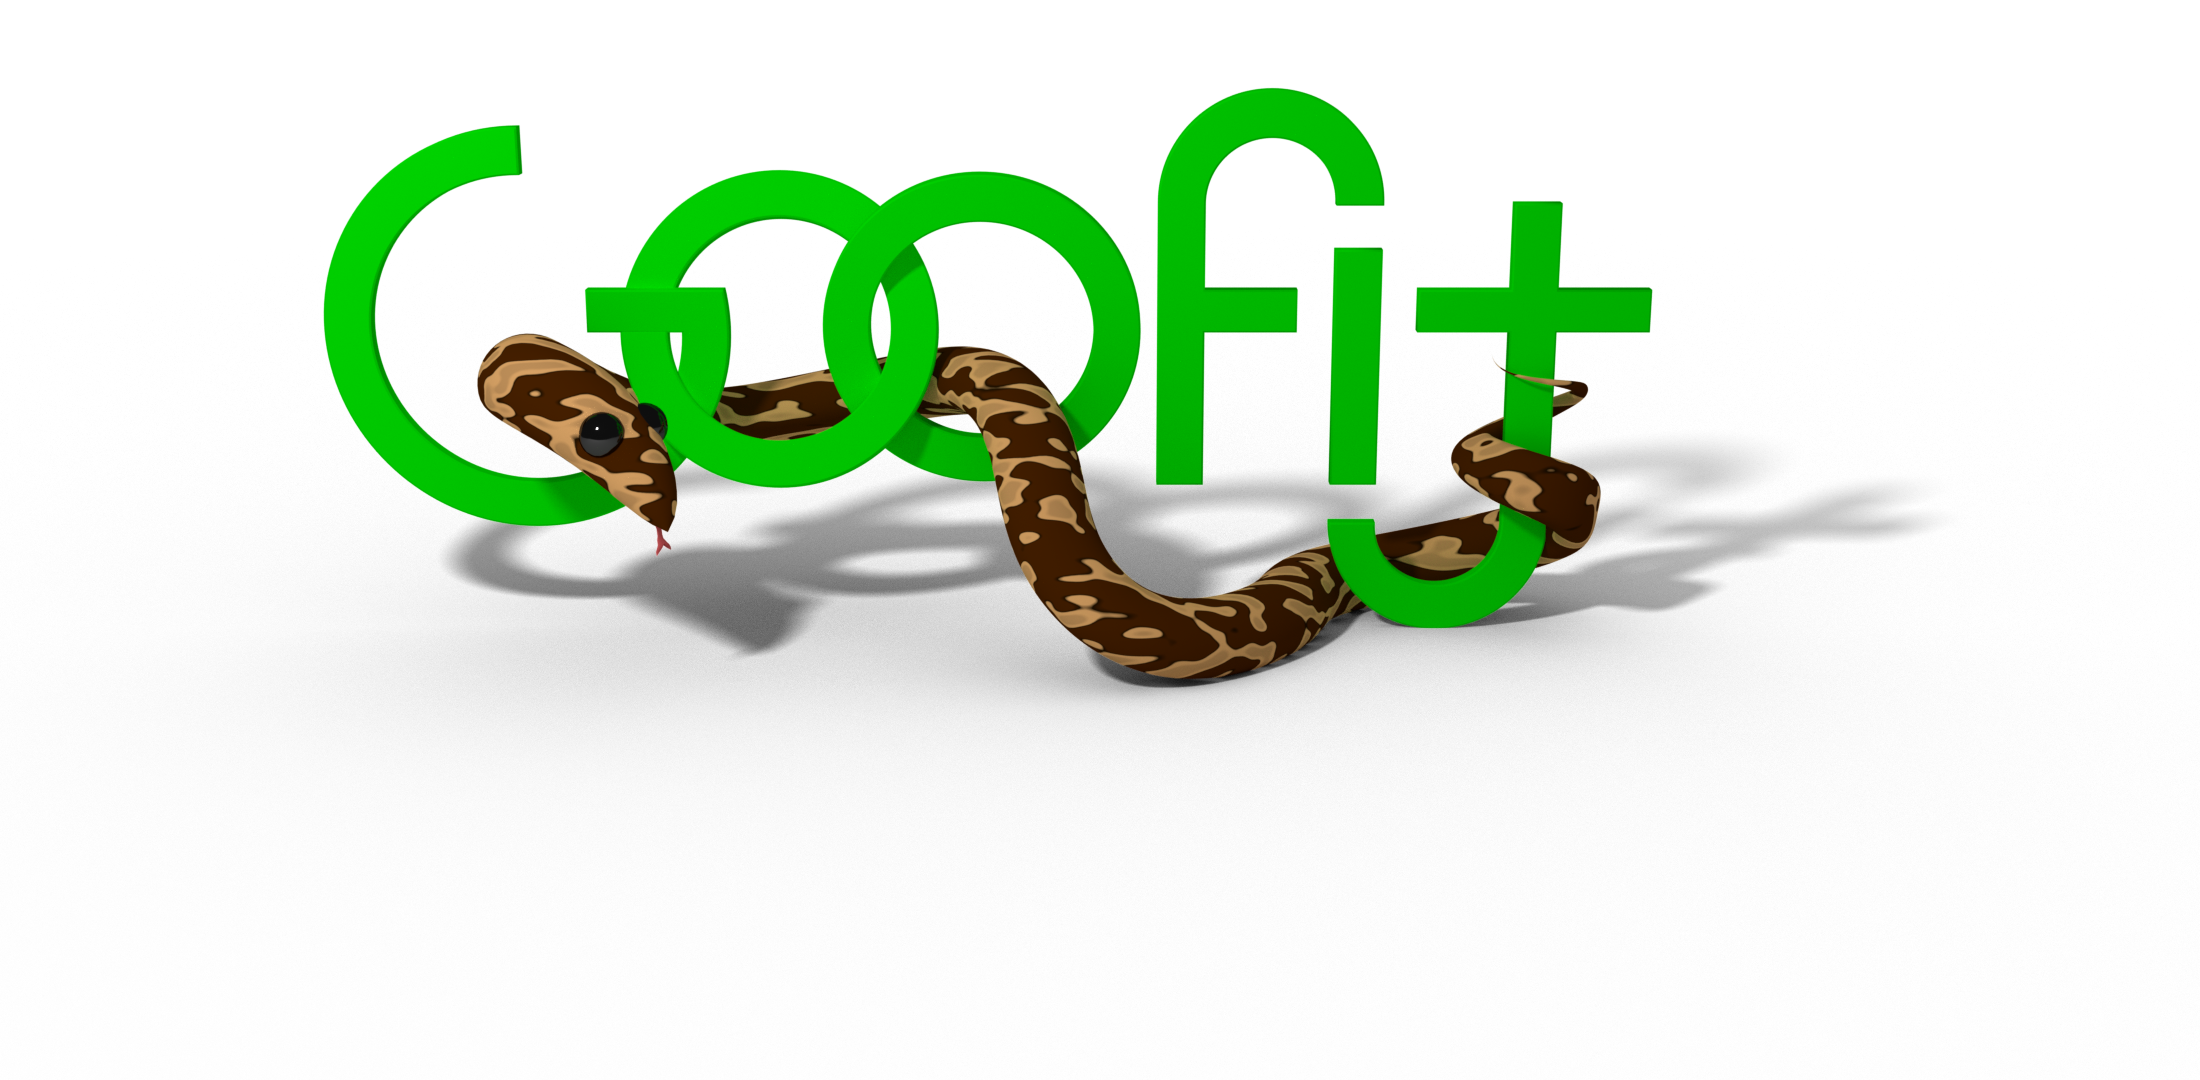
\includegraphics[width=0.5\textwidth]{GooFitSnake}
    \end{center}

    A GPU and OpenMP fitting package designed to look like RooFit, designed for performance.
\end{frame}

\subsection{GooFit Performance}
\begin{frame}{GooFit Performance (2.1)}
\vspace{-.3cm}
\begin{columns}[c]
	\column{.5\textwidth}
	
	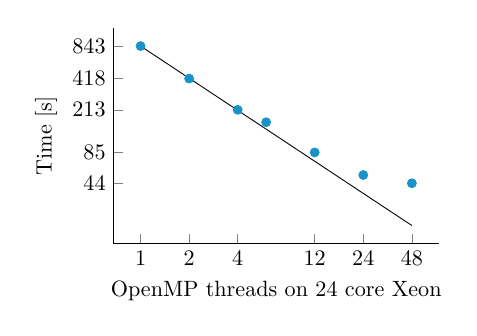
\begin{tikzpicture}[scale=.8]
	\begin{loglogaxis}[
	axis x line*=bottom,
	axis y line*=left,
	xlabel={OpenMP threads on 24 core Xeon},
	ylabel={Time [s]},
	width=6.75cm,
	height=5cm,
	log ticks with fixed point,
	xtick={1,2,4,12,24,48},
	ytick={44,85,213,418,843}
	]
	\addplot[domain=1:48] {843/x};
	\addplot [color=ACATlblue, only marks] coordinates {%
		(1,843)
		(2,418)
		(4, 213)
		(6,163)
		(12, 84.98)
		(24, 52.22)
		(48,43.7)
	};
	
	\end{loglogaxis}
	\end{tikzpicture}
	
	\begin{block}{$\pi\pi\pi^0$, 16 time-dependent amplitudes}
		\begin{itemize}
			%			\item 40 free par.\ and 100,000+ events
			\item Original RooFit code: \unit[19,489]{s} single core
		\end{itemize}
		
		\vspace{-2.5ex}
		\begin{center}
			\begin{tabular}{r|r|l}
				2 Cores & Core 2 Duo &  \unit[1,159]{s} \\
				GPU & GeForce GTX 1050 Ti &  \unit[86.4]{s} \\
				GPU & Tesla K40 & \unit[64.0]{s} \\
				MPI & Tesla K40 $\times 2$ & \unit[39.3]{s} \\
				GPU & Tesla P100 &  \unit[20.3]{s}
				% 3 cards: 34.8 s
				% 2 K-40s: 39.3 s
			\end{tabular}
		\end{center}
	\end{block}
	
	\column{.5\textwidth}
	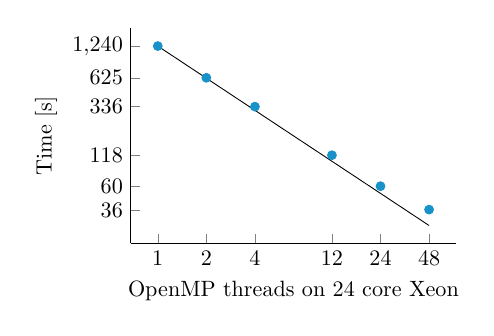
\begin{tikzpicture}[scale=.8]
	\begin{loglogaxis}[
	axis x line*=bottom,
	axis y line*=left,
	xlabel={OpenMP threads on 24 core Xeon},
	ylabel={Time [s]},
	width=6.75cm,
	height=5cm,
	log ticks with fixed point,
	xtick={1,2,4,12,24,48},
	ytick={36, 60, 118, 336, 625, 1240}
	]
	\addplot[domain=1:48] {1239.565/x};
	\addplot [color=ACATlblue, only marks] coordinates {%
		(1,1239.5650)
		(2,625.0800)
		(4,335.6160)
		(12,117.7198)
		(24,60.3316)
		(48,36.4039)
	};
	
	\end{loglogaxis}
	\end{tikzpicture}
	
	\begin{block}{ZachFit: $M (D^{*+})-M (D^0)$}
		\begin{itemize}
			\item 142,576 events in unbinned fit
			%		\item 24 physical Xeon cores for plot(s)
		\end{itemize}
		\vspace{-2.5ex}
		\begin{center}
			\begin{tabular}{r|r|l}
				2 Cores & Core 2 Duo &  \unit[738]{s} \\
				GPU & GeForce GTX 1050 Ti & \unit[60.3]{s} \\
				GPU & Tesla K40 & \unit[96.6]{s} \\
				MPI & Tesla K40 $\times 2$ & \unit[54.3]{s} \\
				GPU & Tesla P100 & \unit[23.5]{s}
			\end{tabular}
		\end{center}
	\end{block}
\end{columns}
\begin{tikzpicture}[overlay, remember picture]
\node at (current page.north east)
[below left, xshift=-1.15cm, yshift=0cm, align=right,font=\footnotesize]
{
	\href{http://inspirehep.net/record/1229331}{[Phys.Rev.Lett. 111 (2013) no.11, 111801]}\\
	\href{http://inspirehep.net/record/1441203/}{[Phys.Rev. D93 (2016) no.11, 112014]}\\
    \href{http://inspirehep.net/record/1228910}{[Phys.Rev. D88 (2013) no.5, 052003]}\\
    \href{http://inspirehep.net/record/1302129}{[CHEP 2013]}
};

 % PPPi_0
 % ZachFit
\end{tikzpicture}
\end{frame}

\subsection{GooFit History}
\begin{frame}{GooFit History}
  
\begin{center}%
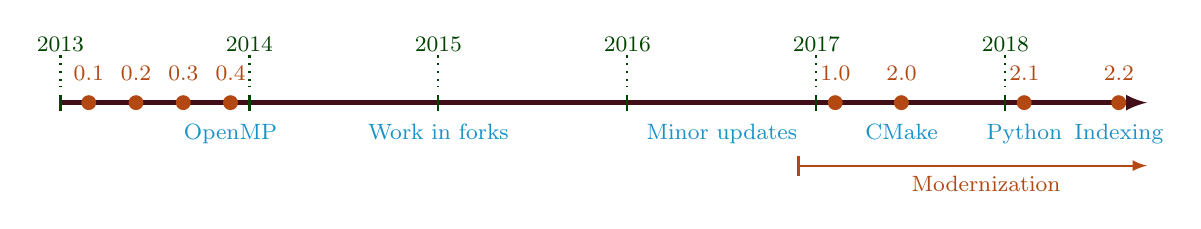
\begin{tikzpicture}[xscale=1.2,
	goonode/.style={fill=ACATdtan, circle, minimum size=1.25ex, inner sep=0},
	version/.style={above=1ex, ACATdtan},
	events/.style={below=1ex, ACATlblue},
	every node/.style={font=\footnotesize}
	]
	\draw [-latex, ultra thick, ACATdbrown] (0,0) -- (11.5,0);
	\draw [|-latex, thick, ACATdtan] (7.8,-.8) -- (11.5,-.8) node [midway, below, xshift=.5em] {Modernization};
	
	\foreach \x in {2013,...,2018} {
		\node at (2*\x-2*2013,0) [above=3.5ex, ACATdgreen] {\x};
		\draw [thick, ACATdgreen] (2*\x-2*2013,-.1) -- (2*\x-2*2013,.1);
		\draw [thick, dotted, ACATdgreen] (2*\x-2*2013,.6) -- (2*\x-2*2013,.2);
	}
	
	\node (v01) at (.3,0) [goonode] {};
	\node at (v01) [version] {0.1};
	
	\node (v02) at (.8,0) [goonode] {};
	\node at (v02) [version] {0.2};
	
	\node (v03) at (1.3,0) [goonode] {};
	\node at (v03) [version] {0.3};
	
	\node (v04) at (1.8,0) [goonode] {};
	\node at (v04) [events] {OpenMP};
	\node at (v04) [version] {0.4};
	
	\node at (4,0) [events] {Work in forks};
	
	\node (v10) at (8.2,0) [goonode] {};
	\node at (7,0) [events] {Minor updates};
	\node at (v10) [version] {1.0};
	
	\node (v20) at (8.9,0)  [goonode] {};
	\node at (v20) [events] {CMake};
	\node at (v20) [version] {2.0};

	\node (v21) at (10.2,0)  [goonode] {};
	\node at (v21) [events] {Python};
	\node at (v21) [version] {2.1};

	\node (v22) at (11.2,0)  [goonode] {};
	\node at (v22) [events] {Indexing};
	\node at (v22) [version] {2.2};
	\end{tikzpicture}%
\end{center}
\vspace{-.5cm}

  \begin{block}{Recent History}
    \begin{itemize}
      \item 2.0: New build system, C++11, and 4-body time dependent analyses support
      \item 2.1: Python bindings
      \item 2.2: New indexing (and lots of Python improvements)
    \end{itemize}
  \end{block}
\end{frame}

\section{GooFit and Python}
\subsection{Installation}
\begin{frame}{Installation}

    \begin{columns}[c]
        \column{.5\textwidth}
        \begin{block}{Pip install}
            \begin{itemize}
                \item Pip always builds from source
                \item Uses CUDA if found, otherwise OpenMP
                \item It is possible to pass in CMake arguments
            \end{itemize}
        \end{block}

        \begin{block}{Pip 9}
            \begin{itemize}
                \item \texttt{pip install skbuild cmake}
                \item \texttt{pip install -v goofit}
            \end{itemize}
        \end{block}

        \begin{block}{Pip 10}
            \begin{itemize}
                \item \texttt{pip install -v goofit}
                \item Note: not a formal endorsement of Pip 10
            \end{itemize}
        \end{block}

        \column{.5\textwidth}

        \begin{block}{CMake and normal directory}
            \begin{itemize}
                \item Build with \texttt{GOOFIT\_PYTHON=ON} (\texttt{Auto} by default)
                \item Build directory should be in path (or install)
            \end{itemize}
        \end{block}
    \end{columns}
\end{frame}


\subsection{Comparison}
\begin{frame}[fragile]{Comparison}
    \begin{columns}[c]
        \column{.5\textwidth}
        \begin{lstlisting}[language=C++]
#include <goofit/...>
using namespace GooFit;

Observable x{"x", 0, 10};
Variable mu{"mu", 1};
Variable sigma{"sigma", 1, 0, 10};
GaussianPdf gauss{"gauss", &x, &mu, &sigma};
// Setup for DataSet ds not shown
gauss.fitTo(&ds);

std::cout << mu << std::endl;
\end{lstlisting}
        \column{.5\textwidth}
        \begin{lstlisting}[language=Python] 
from goofit import *


x = Observable("x", 0, 10)
mu = Variable("mu", 1)
sigma = Variable("sigma", 1, 0, 10)
gauss = GaussianPdf("gauss", x, mu, sigma)
# Setup for DataSet ds not shown
gauss.fitTo(ds)

print(mu)
        \end{lstlisting}
    \end{columns}
\end{frame}

\subsection{Pythonisms}
\begin{frame}[fragile]{Pythonisms}
    \begin{columns}[c]
        \column{.5\textwidth}
        \begin{lstlisting}[language=Python]
mu.value = 2
print(mu)
        \end{lstlisting}
        \begin{block}{Variables}
            \begin{itemize}
                \item Variables provide property access
                \item Variables can be printed
            \end{itemize}
        \end{block}
        \column{.5\textwidth}
        \begin{lstlisting}[language=Python]
import numpy as np 
npdata = np.random.normal(1, 2.5, 100000)
ds = UnbinnedDataSet(xvar)
ds.from_matrix(npdata[:,np.newaxis],
               filter=True)
        \end{lstlisting}
        \begin{block}{DataSet: from Python}
            \begin{itemize}
                \item DataSets can be read in/out to 2D buffers
                \item Auto-filtering invalid values possible
            \end{itemize}
        \end{block}

    \end{columns}
\end{frame}

\subsection{Simulation}
\begin{frame}[fragile]{Simulation}
    \begin{columns}[c]
        \column{.5\textwidth}
        \begin{lstlisting}[language=Python]
grid, pts = gauss.evaluatePdf(x)
gauss.setData(grid)
        \end{lstlisting}
        \begin{block}{PDF evaluation}
            \begin{itemize}
                \item Evaluate on a grid
                \item Can be rerun interactively
            \end{itemize}
        \end{block}

        \begin{lstlisting}[language=Python]
gauss.fillMCDataSimple(1000000)
        \end{lstlisting}
        \begin{block}{MC generation 1D}
            \begin{itemize}
                \item Simple way to produce MC
            \end{itemize}
        \end{block}
        \column{.5\textwidth}
        \begin{lstlisting}[language=Python]
dplt = DalitzPlotter(prod, dp)
arr = dplt.make2D()        
        \end{lstlisting}
        \begin{block}{Amp3Body}
            \begin{itemize}
                \item Can produce simple 3-body Toy MC
                \item DalitzPlotter functionality planned for merge into Amp3Body
            \end{itemize}
        \end{block}

        \begin{lstlisting}[language=Python]
aa.setGenerationOffset(0);
aa.GenerateSig(1000000);
        \end{lstlisting}
        \begin{block}{Amp4Body}
            \begin{itemize}
                \item Full GPU Toy MC using MCBooster
            \end{itemize}
        \end{block}

    \end{columns}
\end{frame}

\subsection{Documentation}
\begin{frame}[fragile]{Documentation}
    \begin{columns}[c]
        \column{.5\textwidth}
        \begin{lstlisting}[language=Python]
import goofit
goofit.MyPdf
        \end{lstlisting}
        % TODO: Add documentation output
        \begin{block}{Documentation}
            \begin{itemize}
                \item Documentation exported to Jupyter
            \end{itemize}
        \end{block}
        \column{.5\textwidth}
        \begin{lstlisting}[language=C++]
.def_static("help", []() {
    return HelpPrinter(MyPdf_docs);
})
        \end{lstlisting}
        \begin{block}{Implementation details}
            \begin{itemize}
                \item Generated by CMake from Doxygen style comments
                \begin{itemize}
                    \item Conversion to Jupyter style markdown for math
                \end{itemize}
                \item Attached to class in PyBind11
            \end{itemize}
        \end{block}
    \end{columns}
\end{frame}

\section{Indexing}
\subsection{How goofit Works}
\begin{frame}
    \begin{columns}[c]
        \column{.65\textwidth}
        \begin{block}{How GooFit Works}
            \begin{itemize}
                \item C++11 classes: Variable and Observable, DataSet, GooPdf
                \item Functions in CUDA with pointers held by GooPdf
                \item Function and variable arrays populated by GooFit
                \item Evaluation runs through CUDA functions through pointers (one kernel)
                \item Launching is handled by Thrust
            \end{itemize}
        \end{block}
        \column{.35\textwidth}
        \begin{center}
            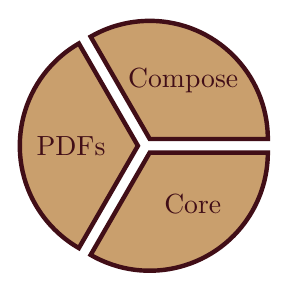
\begin{tikzpicture}
                \path [use as bounding box] (-1.5,-1.5) rectangle (1.5,1.5);
                \begin{scope}[xshift=0.5mm, yshift=0.866mm]
                    \path [ACATdark] (0,0) -- (0:1.5cm) arc (0:120:1.5cm) -- cycle;
                    \node [ACATdarktext] at (60:.85cm) {Compose};
                \end{scope}
                \begin{scope}[xshift=-1mm]
                    \path [ACATdark] (0,0) -- (120:1.5cm) arc (120:240:1.5cm) -- cycle;
                    \node [ACATdarktext] at (180:.85cm) {PDFs};
                \end{scope}
                \begin{scope}[xshift=0.5mm, yshift=-0.866mm]
                    \path [ACATdark] (0,0) -- (240:1.5cm) arc (240:360:1.5cm) -- cycle;
                    \node [ACATdarktext] at (310:.85cm) {Core};
                \end{scope}
            \end{tikzpicture}
        \end{center}
    \end{columns}
\end{frame}


\subsection{Indexing in device functions}
\begin{frame}[fragile]{Indexing in device functions}
\begin{lstlisting}[language=C++]
__device__ fptype f_device(fptype* evt, ParameterContainer& pc) {
    int id       = pc.getObservable(0);
    fptype x     = evt[id];
    fptype v     = pc.getParameter(0);
    pc.incrementIndex(1, 1, 0, 1, 1);
    return x * v;
}

__device__ device_function_ptr ptr_to_Gaussian = device_Gaussian;
\end{lstlisting}

\begin{block}{ParameterContainer}
    \begin{itemize}
        \item Simpler, easier device functions
        \item Faster on GPU, (currently) marginally slower on CPU
    \end{itemize}
\end{block}
\end{frame}

\subsection{Indexing in PDF}
\begin{frame}[fragile]{Indexing in PDF}
\begin{lstlisting}[language=C++]
 __host__ MyPdf::MyPdf(std::string name, Observable x, Variable v,)
     : GooPdf("MyPdf", name, x, v) {
     registerFunction("ptr_to_f", ptr_to_f);
     initialize();
 }
\end{lstlisting}

\begin{block}{Registration}
    \begin{itemize}
        \item Simply register the function (with debug name)
        \item Observables, Variables can be registered in the constructor
    \end{itemize}
\end{block}

\end{frame}


\backupbegin
\section{Backup}

\subsection{Backup slides}

\begin{frame}{Code}
	Code and presentations (as CI artifacts) available at: \url{https://gitlab.cern.ch/hschrein/lhcb_presentation}
\end{frame}

\backupend

\end{document}
